\chapter{Perancangan}
\label{chap:perancangan}
Pada bab ini akan dijelaskan perancangan perangkat lunak yang dibuat pada penelitian ini. Perancangan terdiri dari diagram aktivitas dan masukan perangkat lunak. 

\section{Diagram Aktivitas}
\label{sec:diagramAktivitas}
Perangkat lunak perekaman absen daring otomatis adalah perangkat lunak yang digunakan untuk melakukan absensi secara otomatis bagi mahasiswa UNPAR. Perangkat lunak ini menggunakan Selenium WebDriver sebagai \textit{tools} yang berguna untuk melakukan otomatisasi pada browser web. Perangkat lunak ini juga membutuhkan masukan dari sebuah file konfigurasi untuk menjalankannya.
Diagram Aktivitas untuk \textit{setup} menjalankan program dan menyiapkan file konfigurasi dapat dilihat Gambar \ref{fig:ActivitySetup}. Berikut ini adalah penjelasan langkah-langkah pada diagram aktivitas:
\begin{enumerate}
	\item Pengguna melakukan \textit{install} python, karena program perekaman absen daring otomatis menggunakan bahasa pemrograman python.
	\item Pengguna melakukan \textit{install} selenium, karena untuk melakukan perekaman absen daring secara otomatis menggunakan selenium.
	\item Pengguna melakukan \textit{install} chrome driver, karena menggunakan browser Google Chrome untuk melakukan perekaman absen daring otomatis.
	\item Pengguna membuka file konfigurasi dan mengubah email serta password sesuai milik pengguna agar dapat digunakan sebagai masukan pada perangkat lunak untuk melakukan perekaman absen daring otomatis.
	\item Pengguna menyimpan hasil perubahan yang telah dilakukan pada file konfigurasi.
\end{enumerate}
\begin{figure}[H]
	\centering
	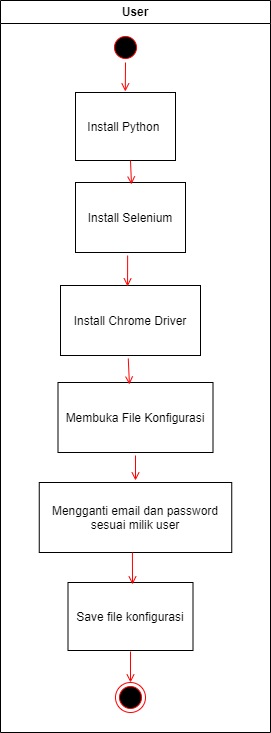
\includegraphics[scale=0.4]{Gambar/ActivitySetup.png}
	\caption{Diagram Aktivitas untuk \textit{Setup} Menjalankan Program} 
	\label{fig:ActivitySetup}
\end{figure}
Diagram Aktivitas untuk perangkat lunak perekaman kehadiran daring otomatis dapat dilihat pada Gambar \ref{fig:ActivityAplikasi}. Berikut ini adalah penjelasan langkah-langkah pada diagram aktivitas:
\begin{enumerate}
	\item Pengguna menjalankan langsung programnya.
	\item WebDriver memberikan perintah untuk membuka browser Google Chrome kepada Driver (Chrome Driver).
	\item Chrome driver disini bertugas menghubungkan setiap perintah dari WebDriver untuk dijalankan pada browser Google Chrome.
	\item Setelah browser Google Chrome terbuka, Browser Google Chrome memberi tahu melalui Chrome driver bahwa perintah sudah dijalankan dan siap menjalankan perintah selanjutnya.
	\item WebDriver memberi perintah membuka web Portal Mahasiswa UNPAR dan Chrome driver memberi tahu kepada browser Google Chrome membuka web Portal Mahasiswa UNPAR.
	\item Browser selanjutnya melakukan login dengan memasukan \textit{email} dan \textit{password} mahasiswa, sesuai dengan perintah dari WebDriver.
	\item Perintah menuju halaman web untuk absensi daring diberikan oleh WebDriver untuk dijalankan secara otomatis oleh Google Chrome.
	\item WebDriver memberi perintah untuk melakukan absensi daring kepada Google Chrome, sehingga dapat terjadi absensi daring secara otomatis.  
	\item Terakhir WebDriver memberi perintah untuk menutup browser Google Chrome setelah berhasil melakukan absensi dan browser Google Chrome ditutup secara otomatis.
\end{enumerate}
\begin{figure}[H]
	\centering
	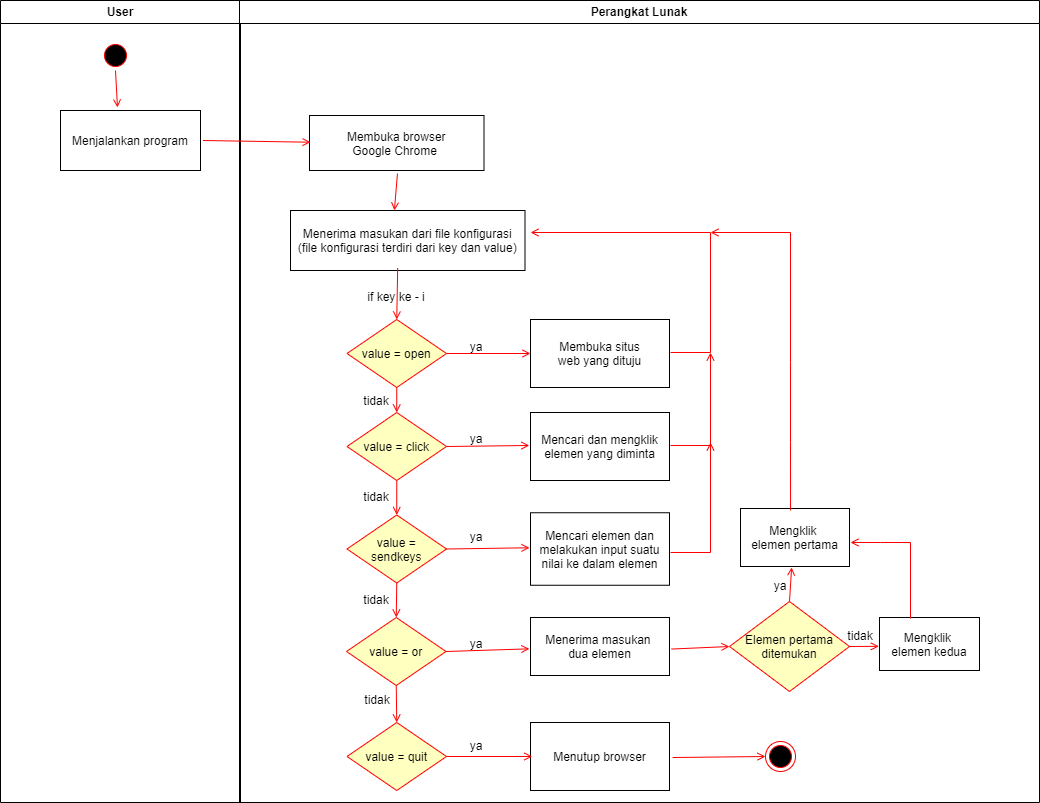
\includegraphics[scale=0.4]{Gambar/ActivityAplikasi.png}
	\caption{Diagram Aktivitas Perangkat Lunak Absen Daring Otomatis} 
	\label{fig:ActivityAplikasi}
\end{figure}

\section{Masukan Perangkat Lunak}
\label{sec:inputConfig} 
Perangkat lunak perekaman kehadiran daring otomatis membutuhkan 1 file sebagai masukan, yaitu \textit{file} .ini (\textit{file} konfigurasi). Pada \textit{file} .ini, nomor baris sebagai \textit{keys} dan \textit{string} berupa kata yang merupakan fungsi dari Selenium WebDriver dan elemen yang diambil untuk melakukan perekaman kehadiran daring otomatis sebagai \textit{values}. Contoh \textit{file} .ini dapat dilihat pada Listing \ref{kode:4:conf}.
\begin{lstlisting}[caption=Contoh \textit{file} .ini untuk Masukan Perangkat Lunak Perekaman Kehadiran Daring Otomatis, label=kode:4:conf]
	[database_config]
	1 = open https://studentportal.unpar.ac.id
	2 = click #login-button
	3 = sendkeys #username 2017730035@student.unpar.ac.id 
	4 = quit
\end{lstlisting}
Berikut ini penjelasan dari isi dari contoh \textit{file} .ini:
\begin{itemize}
	\item Baris pertama berisi nama \textit{section} untuk isi \textit{file} .ini.
	\item \textit{keys} pada \textit{file} .ini ini pasti berupa angka yang terurut agar perangkat lunak dapat menjalankannya secara terurut.
	\item Terdapat 4 fungsi kata dari Selenium WebDriver, yaitu \textit{open}, \textit{click}, \textit{sendkeys}, dan \textit{quit}.
	\item \textit{Keys} 1 pasti diisi oleh fungsi \textit{open}, lalu diisi situs web yang ingin dibuka (\url{https://studentportal.unpar.ac.id}), karena langkah pertama setelah berhasil membuka browser adalah menuju pada situs web yang akan diotomatisasi.
	\item \textit{Keys} 2 memiliki fungsi \textit{click} untuk menekan tombol secara otomatis dan diisi elemen ``\#login-button'' yang diambil berdasarkan CSS Selector.
	\item \textit{Keys} 3 memiliki fungsi \textit{sendkeys} untuk memasukan suatu nilai ke dalam elemen yang dipilih, yaitu elemen ``\#username'' dan isinya adalah ``2017730035@student.unpar.ac.id''.
	\item \textit{Keys} 4 memiliki fungsi \textit{quit} untuk menutup browsernya.
\end{itemize}
Elemen yang dipakai dalam \textit{file} .ini ini diambil dengan cara melakukan \textit{inspect element} pada web yang ingin dilakukan otomatisasi. Pada Gambar \ref{fig:inspect} adalah cara yang dilakukan untuk mendapat elemen yang ingin digunakan untuk melakukan otomatisasi. Untuk mendapatkan elemen tersebut, perlu melakukan klik kanan pada bagian elemen yang ingin diambil, lalu pilih ``inspect''. Setelah melakukan ``inspect'' maka akan muncul dokumen HTML yang dapat dilihat pada bagian kanan Gambar \ref{fig:inspect}, sehingga dapat melakukan pengambilan elemen yang diperlukan.
\begin{figure}[H]
	\centering
	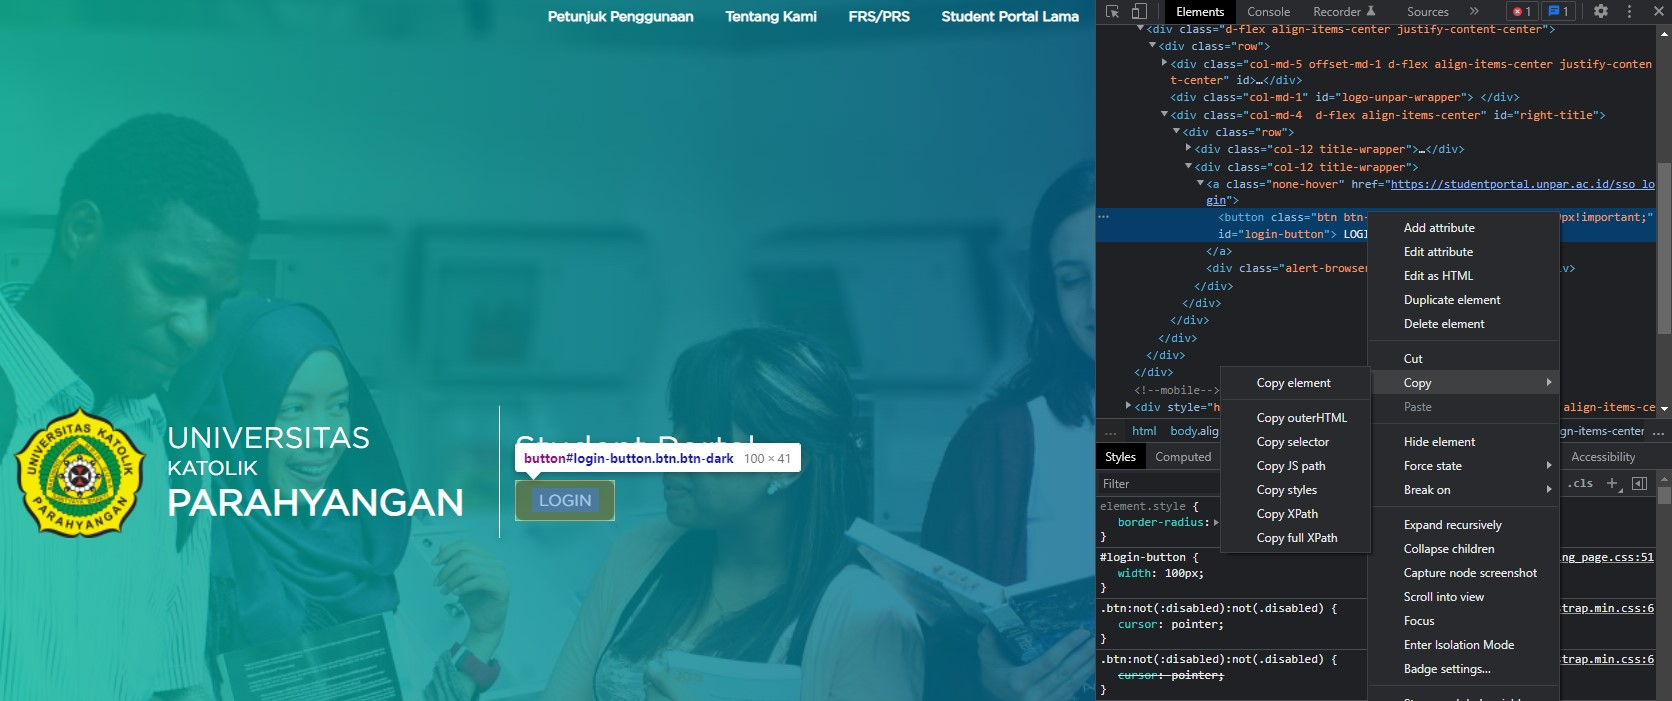
\includegraphics[scale=0.4]{Gambar/elemen.jpg}
	\caption{Tampilan Melakukan \textit{Inspect Element}} 
	\label{fig:inspect}
\end{figure}	